\documentclass[conference]{IEEEtran}
\usepackage[utf8]{inputenc}
\usepackage{cite,graphicx,booktabs,tabularx,array,url}
\newcolumntype{Y}{>{\raggedright\arraybackslash}X}
\begin{document}

\title{Toward Smart Glasses: A Grounded Voice Interactive Object Assistant Prototyped on Meta Quest 3}
\author{\IEEEauthorblockN{Lakshya Singh}
\IEEEauthorblockA{Student\\CSE Department\\SRM University-AP\\Amaravati, India}
\and
\IEEEauthorblockN{Om Mittal}
\IEEEauthorblockA{Student\\CSE Department\\SRM University-AP\\Amaravati, India}
\and
\IEEEauthorblockN{Darpan Mondal}
\IEEEauthorblockA{Student\\CSE Department\\SRM University-AP\\Amaravati, India}
\and
\IEEEauthorblockN{Atmakuri Yeshwanth}
\IEEEauthorblockA{Student\\CSE Department\\SRM University-AP\\Amaravati, India}
\and
\IEEEauthorblockN{M. Abdussami}
\IEEEauthorblockA{Assistant Professor\\CSE Department\\SRM University-AP\\Amaravati, India}}
\maketitle

\begin{abstract}
This paper presents an extension of an existing Unity mixed reality object detection project into a voice interactive assistant. The intended future form factor is camera equipped smart glasses; Meta Quest 3 served as the available development and validation platform because the required camera access, inference stack, and test hardware were available there. A bundled YOLO12n model runs through Unity Sentis on camera frames. Detected labels, counts, screen relative positions, and approximate colors become a structured scene snapshot. Deterministic rules answer direct visual questions, while a PC gateway routes organization requests to Google AI and speech input/output to ElevenLabs. Model proposed actions are checked against current detection indices before being spoken. In offline validation, all 36 Unity Edit Mode tests and six gateway tests passed. Manual Quest 3 checks confirmed live detections and several spoken inventory and count answers. The evaluation does not establish detector accuracy, frame rate, power use, or performance on smart glasses; these require controlled measurements. The contribution is a small, grounded end to end prototype with explicit uncertainty when visual evidence is insufficient.
\end{abstract}

\begin{IEEEkeywords}
mixed reality, object detection, voice assistant, visual grounding, Meta Quest 3
\end{IEEEkeywords}

\section{Introduction}
Wearable visual assistants promise hands free access to nearby objects, but spoken answers must remain tied to what the camera actually detects. Object detection has advanced from YOLO to mobile friendly networks and transformer detectors \cite{yolo,coco,mobilenet,rtdetr}. Meta's Quest 3 camera interface and Unity Sentis provide a practical development platform \cite{meta,unity}. This work targets a future glasses shaped assistant, while the present prototype uses Quest 3 because its supported camera API and on device ML path could be implemented and tested within the project constraints. No experiment on smart glasses is claimed.

The contribution is an integration of the existing project rather than a new detector or training method:
\begin{itemize}
\item a current frame scene representation with class, count, screen zone, and cautious color estimates;
\item a question router that answers direct visual queries locally and validates AI placement actions against observed detections;
\item an operational speech and reasoning path with cloud credentials held by a PC gateway, plus a compact Quest interface.
\end{itemize}
Section II reviews recent methods. Section III describes the architecture and working flow. Section IV reports reproducible checks and their limits. Section V concludes.

\section{Literature Review}
Recent detectors improve efficiency or open vocabulary coverage, while vision language models broaden question answering. Table~\ref{tab:survey} compares twelve papers published in 2024--2025 \cite{yolov9,yolov10,yolov12,yoloworld,groundingdino15,florence2,mobileclip,mobilevlmv2,paligemma,llavaonevision,qwen2vl,molmo}. Reported outcomes in the table belong to the cited papers; none is a measured result of this prototype.

\begin{table*}[t]
\caption{Recent literature survey. ``Difference'' describes the present prototype, not a reproduced benchmark.}
\label{tab:survey}
\centering\scriptsize\setlength{\tabcolsep}{3pt}\renewcommand{\arraystretch}{1.12}
\begin{tabularx}{\textwidth}{@{}llYYYYY@{}}
\toprule
Ref. & Year & Methodology & Dataset / evaluation & Key result reported & Limitation for this task & Difference in proposed work \\
\midrule
\cite{yolov9} & 2024 & PGI and GELAN detector & COCO & Better accuracy--efficiency tradeoff & Detector without voice QA & Uses fixed detector with spoken queries \\
\cite{yolov10} & 2024 & NMS free end to end YOLO & COCO & Lower inference latency & No scene dialogue & Adds grounded scene answers \\
\cite{yolov12} & 2025 & Attention centric YOLO & COCO & Strong speed--accuracy balance & No Quest speech workflow & Deploys bundled nano variant in Unity \\
\cite{yoloworld} & 2024 & Open vocabulary real time YOLO & LVIS, COCO & Detects text specified classes & Larger open vocabulary pipeline & Uses 80 known labels and explicit abstention \\
\cite{groundingdino15} & 2024 & Open set grounding detector & COCO, LVIS & Strong open set AP & Edge variant still needs integration & Uses on headset closed set inference \\
\cite{florence2} & 2024 & Unified vision foundation model & FLD-5B; vision tasks & Transfers across tasks & General model, heavier workflow & Separates compact detection from reasoning \\
\cite{mobileclip} & 2024 & Efficient image--text encoder & ImageNet; retrieval & Competitive mobile zero shot transfer & No boxes or speech response & Uses localized detections and TTS \\
\cite{mobilevlmv2} & 2024 & Mobile vision language model & ShareGPT4V, ScienceQA, TextVQA & Small model competes with larger VLMs & No Quest camera validation & Uses structured scene rather than raw image VLM \\
\cite{paligemma} & 2024 & Transferable 3B vision language model & RefCOCO, DocVQA and others & Broad transfer to visual tasks & Not evaluated on Quest & Runs only compact detector on Quest \\
\cite{llavaonevision} & 2024 & Image and video multimodal model & MMMU, MMBench, video tasks & Cross scenario transfer & Not constrained to current detection IDs & Validates each suggested action \\
\cite{qwen2vl} & 2024 & Resolution adaptive VLM & DocVQA, MMBench, MathVista & Strong multimodal perception & Larger model; no local Quest test & Uses lightweight local perception \\
\cite{molmo} & 2025 & Open vision language model & PixMo and VLM benchmarks & Strong open model grounding & Not a speech headset system & Couples detected objects to spoken output \\
\bottomrule
\end{tabularx}
\end{table*}

Related efficient and multimodal work includes segmentation \cite{sam,efficientsam,efficientvitsam,sam2}, compact vision language models \cite{clip,tinyllava,smolvlm,vila,paligemma2,florencevl,dinox}, and streaming speech synthesis \cite{whisper,cosyvoice,cosyvoice2}. Visual hallucination studies motivate strict evidence checks \cite{pope,hallusionbench,faithscore,woodpecker}; long context multimodal reasoning motivates optional cloud planning \cite{gemini15}. These works were not run as baselines in this project.

\section{Methodology}
Fig.~\ref{fig:block} shows the implemented blocks. Quest 3 supplies camera frames and microphone input. The Meta XR object detection block executes a bundled \texttt{yolo12nNoNMS.sentis} model through Unity Sentis. Its profile specifies 640$\times$640 input, 80 class labels, a 0.5 score threshold, at most 100 detections, and work split across frames. The class list follows a COCO style taxonomy; the repository does not document the model's original training split. A scene builder stores each detection's label, confidence, box, index, and screen relative zone. It estimates a color only when a 5$\times$5 central pixel sample has sufficient saturation and a dominant hue vote; otherwise the color remains unknown.

\begin{figure*}[t]
\centering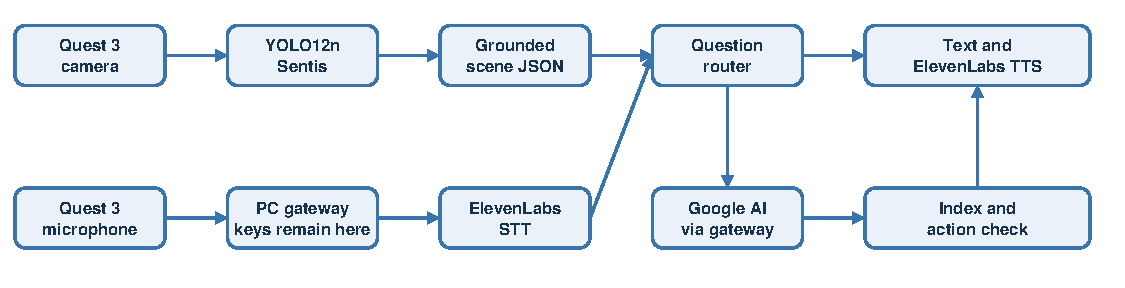
\includegraphics[width=0.96\textwidth]{figures/block_diagram.pdf}
\caption{Block diagram of the Quest perception path and the PC gateway. Editable source: \texttt{figures/block\_diagram.drawio}.}
\label{fig:block}
\end{figure*}

Fig.~\ref{fig:flow} shows the request flow. Pressing X begins speech recognition; Y requests a preset visible object inventory. Each question uses a fresh detection snapshot. Direct inventory, count, color, and screen location questions are answered by deterministic code using that snapshot. Organization requests go through a PC REST gateway to Google AI, which returns action JSON. Allowed actions are left, right, center, group, and separate; object and target indices must refer to current detections. Empty or invalid plans yield an uncertainty response. The panel shows microphone, detection, AI, and connection states, while the response is synthesized using the existing Meta/ElevenLabs speech block. Google and ElevenLabs keys are read on the PC, not stored in Unity assets.

\begin{figure*}[t]
\centering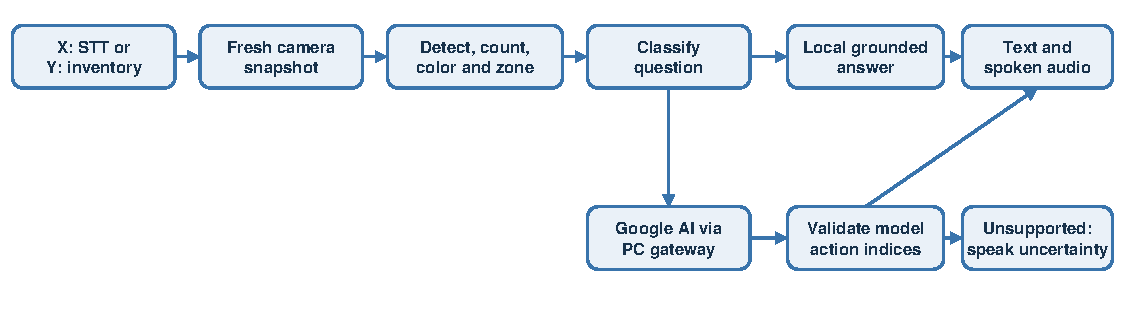
\includegraphics[width=0.96\textwidth]{figures/working_flow.pdf}
\caption{Working flow for preset and spoken queries. Editable source: \texttt{figures/working\_flow.drawio}.}
\label{fig:flow}
\end{figure*}

\section{Experimental Setup and Results}
\subsection{Experimental Setup}
The prototype uses Unity 6 (6000.3.19f1), Meta XR SDK 85.0.0, Sentis 2.6.1, Quest 3, and a Python gateway. The configured Google path is a Gemini model; speech profiles use ElevenLabs Scribe v1 and Flash v2.5. No detector training, fine tuning, dataset partition, or train/test split was performed in this repository. Offline inputs were a synthetic 640$\times$640 gray texture for an inference smoke test and constructed object/100$\times$100 color scenes for logic tests. Metrics reported here are test pass counts, test fixture wall time, and artifact size. These are software verification measures, not COCO mAP or device inference latency. No controlled detector baseline or ablation experiment was run. Project source, tests, and the PC gateway are available at \url{https://github.com/lakshya-02/Object-Detection}.

Table~\ref{tab:tests} and Figs.~\ref{fig:counts}--\ref{fig:times} summarize the archived Unity Test Framework XML. That Edit Mode run passed 36/36 cases; the 23.38~s model smoke case includes Editor test overhead and must not be read as per frame latency. A final Edit Mode run on November 18 also passed 36/36 cases; its XML is supplied separately.
\begin{table}[t]
\caption{Unity Edit Mode results from saved test XML}
\label{tab:tests}\centering\footnotesize
\begin{tabular}{@{}lrr@{}}\toprule
Fixture & Pass/total & Time (s) \\ \midrule
Scene context & 32/32 & 0.027 \\
Model inference smoke & 1/1 & 23.385 \\
Scene wiring & 1/1 & 0.471 \\
UI output & 1/1 & 0.055 \\
Gateway request & 1/1 & 0.019 \\
\midrule All & 36/36 & 23.964 \\ \bottomrule
\end{tabular}
\end{table}

\begin{figure}[t]
\centering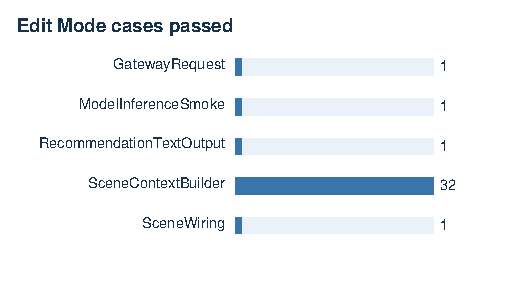
\includegraphics[width=\columnwidth]{figures/test_counts.pdf}
\caption{Passed Edit Mode cases by fixture; this counts software tests, not detected objects.}
\label{fig:counts}
\end{figure}
\begin{figure}[t]
\centering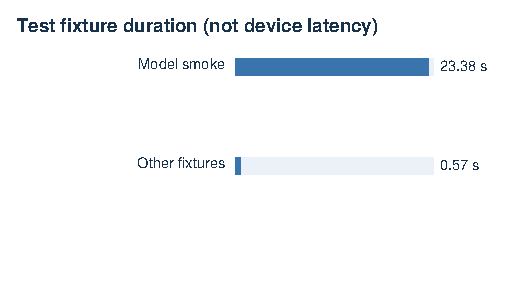
\includegraphics[width=\columnwidth]{figures/test_times.pdf}
\caption{Saved fixture durations; the smoke test duration includes Editor overhead.}
\label{fig:times}
\end{figure}

Table~\ref{tab:queries} records representative deterministic checks against constructed scenes. These verify answer grounding under the stated inputs, not open world accuracy.
\begin{table}[t]
\caption{Constructed scene question checks}
\label{tab:queries}\centering\footnotesize
\begin{tabularx}{\columnwidth}{@{}YYY@{}}\toprule
Scene input & Question type & Verified response \\ \midrule
Two books & Count & ``2 books'' \\
Laptop + TV & Multi class count & Both counts \\
Yellow/green objects & Color + zone & Distinct labels \\
Book; no pen & Missing object & Declines pen claim \\
Invalid action index & Placement & Declines plan \\ \bottomrule
\end{tabularx}
\end{table}

Table~\ref{tab:gateway} summarizes six Python gateway tests using mocked upstream responses and substitute credentials. Prior manual Quest 3 checks showed live labels, spoken Y inventory, and spoken X count answers for a visible TV class. On November 18, the final APK was installed and launched without a reported crash; a user wearing Quest 3 confirmed live labels, text, and spoken replies from both X and Y. The gateway recorded successful text to speech requests. These are informal functional observations, not a timed or randomized accuracy trial.
\begin{table}[t]
\caption{PC gateway verification, mocked cloud upstream}
\label{tab:gateway}\centering\footnotesize
\begin{tabularx}{\columnwidth}{@{}YcY@{}}\toprule
Check group & Cases & Result \\ \midrule
Google request and JSON envelope & 3 & Pass \\
ElevenLabs key forwarding & 1 & Pass \\
Malformed upstream response & 1 & HTTP 502 \\
Client allowlist & 1 & HTTP 403 \\ \bottomrule
\end{tabularx}
\end{table}

Table~\ref{tab:resource} and Fig.~\ref{fig:size} report file footprint. A prior ten second Quest trace contained no usable app frame intervals. Thus FPS, CPU/GPU utilization, power, memory, mAP, and color accuracy remain unmeasured; no comparison or training curve is presented as if measured.
\begin{table}[t]
\caption{Artifact footprint and missing device metrics}
\label{tab:resource}\centering\footnotesize
\begin{tabular}{@{}lrl@{}}\toprule
Measure & Value & Basis \\ \midrule
Bundled model & 2.91 MB & File size \\
Quest APK & 98.58 MB & File size \\
Quest FPS & N/M & No frame intervals \\
Power / memory & N/M & No instrumented run \\ \bottomrule
\end{tabular}
\end{table}
\begin{figure}[t]
\centering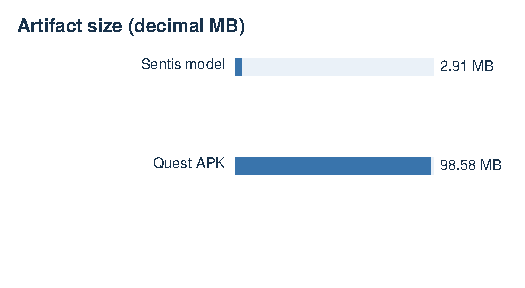
\includegraphics[width=\columnwidth]{figures/artifact_sizes.pdf}
\caption{Measured decimal file sizes; APK size includes assets and runtime.}
\label{fig:size}
\end{figure}

\section{Conclusion}
The existing Unity project now demonstrates a grounded spoken object assistant on Quest 3. It distinguishes current detections from unsupported claims, handles direct questions locally, and validates AI placement actions. The evidence supports software test success and selected manual speech interactions, but not detector accuracy, stable frame rate, power efficiency, or transfer to smart glasses. Future work is a controlled multi object Quest trial with labeled ground truth, latency and power logging, baseline/ablation comparisons, and eventual testing on camera capable smart glasses when an appropriate platform is available.

\section*{Acknowledgment}
AI assisted writing and diagram drafting were used in preparing this manuscript. The authors are responsible for checking all claims, references, and final experimental evidence before submission.

\begin{thebibliography}{99}
\bibitem{yolo} Joseph Redmon et al., ``You Only Look Once: Unified, Real-Time Object Detection,'' \emph{Proc. IEEE/CVF CVPR}, 2016, doi: \url{https://doi.org/10.1109/CVPR.2016.91}.
\bibitem{coco} Tsung-Yi Lin et al., ``Microsoft COCO: Common Objects in Context,'' \emph{Lecture notes in computer science}, 2014, doi: \url{https://doi.org/10.1007/978-3-319-10602-1_48}.
\bibitem{mobilenet} Andrew Howard et al., ``MobileNets: Efficient Convolutional Neural Networks for Mobile Vision Applications,'' \emph{arXiv preprint}, 2017, doi: \url{https://doi.org/10.48550/arxiv.1704.04861}.
\bibitem{rtdetr} Yian Zhao et al., ``DETRs Beat YOLOs on Real-time Object Detection,'' \emph{Proc. IEEE/CVF CVPR}, 2024, doi: \url{https://doi.org/10.1109/CVPR52733.2024.01605}.
\bibitem{meta} Meta, ``Passthrough Camera API Overview for Unity,'' 2026. [Online]. Available: \url{https://developers.meta.com/vr/documentation/unity/unity-pca-overview/}. Accessed: Nov. 18, 2026.
\bibitem{unity} Unity Technologies, ``Sentis 2.6.1 Overview,'' 2026. [Online]. Available: \url{https://docs.unity.cn/Packages/com.unity.ai.inference@2.6/manual/index.html}. Accessed: Nov. 18, 2026.
\bibitem{yolov9} Chien-Yao Wang et al., ``YOLOv9: Learning What You Want to Learn Using Programmable Gradient Information,'' \emph{Lecture notes in computer science}, 2024, doi: \url{https://doi.org/10.1007/978-3-031-72751-1_1}.
\bibitem{yolov10} Ao Wang et al., ``YOLOv10: Real-Time End-to-End Object Detection,'' \emph{Proc. NeurIPS}, 2024, doi: \url{https://doi.org/10.52202/079017-3429}.
\bibitem{yolov12} Yunjie Tian et al., ``YOLOv12: Attention-Centric Real-Time Object Detectors,'' \emph{Proc. NeurIPS}, 2025, doi: \url{https://doi.org/10.52202/085713-2627}.
\bibitem{yoloworld} Tianheng Cheng et al., ``YOLO-World: Real-Time Open-Vocabulary Object Detection,'' \emph{Proc. IEEE/CVF CVPR}, 2024, doi: \url{https://doi.org/10.1109/cvpr52733.2024.01599}.
\bibitem{groundingdino15} Tianhe Ren et al., ``Grounding DINO 1.5: Advance the "Edge" of Open-Set Object Detection,'' \emph{arXiv preprint}, 2024, doi: \url{https://doi.org/10.48550/arxiv.2405.10300}.
\bibitem{florence2} Bin Xiao et al., ``Florence-2: Advancing a Unified Representation for a Variety of Vision Tasks,'' \emph{Proc. IEEE/CVF CVPR}, 2024, doi: \url{https://doi.org/10.1109/cvpr52733.2024.00461}.
\bibitem{mobileclip} Pavan Kumar Anasosalu Vasu et al., ``MobileCLIP: Fast Image-Text Models through Multi-Modal Reinforced Training,'' \emph{Proc. IEEE/CVF CVPR}, 2024, doi: \url{https://doi.org/10.1109/cvpr52733.2024.01511}.
\bibitem{mobilevlmv2} Xiangxiang Chu et al., ``MobileVLM V2: Faster and Stronger Baseline for Vision Language Model,'' \emph{arXiv preprint}, 2024, doi: \url{https://doi.org/10.48550/arxiv.2402.03766}.
\bibitem{paligemma} Lucas Beyer et al., ``PaliGemma: A versatile 3B VLM for transfer,'' \emph{arXiv preprint}, 2024, doi: \url{https://doi.org/10.48550/arxiv.2407.07726}.
\bibitem{llavaonevision} Bo Li et al., ``LLaVA-OneVision: Easy Visual Task Transfer,'' \emph{arXiv preprint}, 2024, doi: \url{https://doi.org/10.48550/arxiv.2408.03326}.
\bibitem{qwen2vl} Peng Wang et al., ``Qwen2-VL: Enhancing Vision-Language Model's Perception of the World at Any Resolution,'' \emph{arXiv preprint}, 2024, doi: \url{https://doi.org/10.48550/arxiv.2409.12191}.
\bibitem{molmo} Matt Deitke et al., ``Molmo and PixMo: Open Weights and Open Data for State-of-the-Art Vision-Language Models,'' \emph{Proc. IEEE/CVF CVPR}, 2025, doi: \url{https://doi.org/10.1109/cvpr52734.2025.00018}.
\bibitem{sam} Alexander Kirillov et al., ``Segment Anything,'' \emph{IEEE/CVF International Conference on Computer Vision (ICCV)}, 2023, doi: \url{https://doi.org/10.1109/iccv51070.2023.00371}.
\bibitem{efficientsam} Yunyang Xiong et al., ``EfficientSAM: Leveraged Masked Image Pretraining for Efficient Segment Anything,'' \emph{Proc. IEEE/CVF CVPR}, 2024, doi: \url{https://doi.org/10.1109/cvpr52733.2024.01525}.
\bibitem{efficientvitsam} Zhuoyang Zhang et al., ``EfficientViT-SAM: Accelerated Segment Anything Model Without Performance Loss,'' \emph{Proc. IEEE/CVF CVPR}, 2024, doi: \url{https://doi.org/10.1109/cvprw63382.2024.00782}.
\bibitem{sam2} Nikhila Ravi et al., ``SAM 2: Segment Anything in Images and Videos,'' \emph{arXiv preprint}, 2024, doi: \url{https://doi.org/10.48550/arxiv.2408.00714}.
\bibitem{clip} Alec Radford et al., ``Learning Transferable Visual Models From Natural Language Supervision,'' \emph{arXiv preprint}, 2021, doi: \url{https://doi.org/10.48550/arxiv.2103.00020}.
\bibitem{tinyllava} Baichuan Zhou et al., ``TinyLLaVA: A Framework of Small-scale Large Multimodal Models,'' \emph{arXiv preprint}, 2024, doi: \url{https://doi.org/10.48550/arxiv.2402.14289}.
\bibitem{smolvlm} Andres Marafioti et al., ``SmolVLM: Redefining small and efficient multimodal models,'' \emph{arXiv preprint}, 2025, doi: \url{https://doi.org/10.48550/arxiv.2504.05299}.
\bibitem{vila} Ji Lin et al., ``VILA: On Pre-training for Visual Language Models,'' \emph{Proc. IEEE/CVF CVPR}, 2024, doi: \url{https://doi.org/10.1109/cvpr52733.2024.02520}.
\bibitem{paligemma2} Steiner, Andreas et al., ``PaliGemma 2: A Family of Versatile VLMs for Transfer,'' \emph{arXiv preprint}, 2024, doi: \url{https://doi.org/10.48550/arxiv.2412.03555}.
\bibitem{florencevl} Jiuhai Chen et al., ``Florence-VL: Enhancing Vision-Language Models with Generative Vision Encoder and Depth-Breadth Fusion,'' \emph{Proc. IEEE/CVF CVPR}, 2025, doi: \url{https://doi.org/10.1109/cvpr52734.2025.02321}.
\bibitem{dinox} Tianhe Ren et al., ``DINO-X: A Unified Vision Model for Open-World Object Detection and Understanding,'' \emph{arXiv preprint}, 2024, doi: \url{https://doi.org/10.48550/arxiv.2411.14347}.
\bibitem{whisper} Alec Radford et al., ``Robust Speech Recognition via Large-Scale Weak Supervision,'' \emph{arXiv preprint}, 2022, doi: \url{https://doi.org/10.48550/arxiv.2212.04356}.
\bibitem{cosyvoice} Zhihao Du et al., ``CosyVoice: A Scalable Multilingual Zero-shot Text-to-speech Synthesizer based on Supervised Semantic Tokens,'' \emph{arXiv preprint}, 2024, doi: \url{https://doi.org/10.48550/arxiv.2407.05407}.
\bibitem{cosyvoice2} Zhihao Du et al., ``CosyVoice 2: Scalable Streaming Speech Synthesis with Large Language Models,'' \emph{arXiv preprint}, 2024, doi: \url{https://doi.org/10.48550/arxiv.2412.10117}.
\bibitem{pope} Yifan Li et al., ``Evaluating Object Hallucination in Large Vision-Language Models,'' \emph{Conference on Empirical Methods in Natural Language Processing (EMNLP)}, 2023, doi: \url{https://doi.org/10.18653/v1/2023.emnlp-main.20}.
\bibitem{hallusionbench} Tianrui Guan et al., ``Hallusionbench: An Advanced Diagnostic Suite for Entangled Language Hallucination and Visual Illusion in Large Vision-Language Models,'' \emph{Proc. IEEE/CVF CVPR}, 2024, doi: \url{https://doi.org/10.1109/cvpr52733.2024.01363}.
\bibitem{faithscore} Liqiang Jing et al., ``FaithScore: Fine-grained Evaluations of Hallucinations in Large Vision-Language Models,'' \emph{Findings of EMNLP}, 2024, doi: \url{https://doi.org/10.18653/v1/2024.findings-emnlp.290}.
\bibitem{woodpecker} Shukang Yin et al., ``Woodpecker: hallucination correction for multimodal large language models,'' \emph{Science China Information Sciences}, 2024, doi: \url{https://doi.org/10.1007/s11432-024-4251-x}.
\bibitem{gemini15} Gemini Team et al., ``Gemini 1.5: Unlocking multimodal understanding across millions of tokens of context,'' \emph{arXiv preprint}, 2024, doi: \url{https://doi.org/10.48550/arxiv.2403.05530}.

\end{thebibliography}
\end{document}
